% ||||||||||||||||||||||||||||||||||||||||||||||
% Capitulo de Revisão Bibliográfica
% ||||||||||||||||||||||||||||||||||||||||||||||

\chapter{Revisão Bibliográfica}

Com o objetivo de compreender os conceitos básicos do trabalho, este capítulo os apresenta de forma evolutiva e 
cronológica, partindo dos conceitos sobre motores elétricos com suas particularidades, até o estado da arte em 
detecção e diagnóstico de falhas em motores elétricos de indução. 


%++++++++++++++++++++++++++++++++++++++++++++++++++++++++++++++++
% 
%++++++++++++++++++++++++++++++++++++++++++++++++++++++++++++++++

\section{Motores Elétricos de Indução}\label{sec:}

Motores elétricos de indução são um dos tipos de máquinas elétricas, as quais convertem energia elétrica em mecânica. 
Nos motores elétricos de indução, uma corrente elétrica é induzida no rotor através da corrente de armadura que circula
no estator. Contudo, um rotor do tipo gaiola de esquilo, pode ser visto na figura \ref{fig:ind_motor_petruzella_p115}, 
é um curto-circuito formado por barras e lâminas de alumínio. Por essa constituição simples, motores elétricos de indução
com rotor do tipo gaiola resultam em motores relativamente baratos e confiáveis, contribuindo para sua popularidade \cite{Umans2003}.
 
\begin{figure}[H]
    \caption{Motor elétrico de indução tipo gaiola de esquilo.}
    \begin{center}
        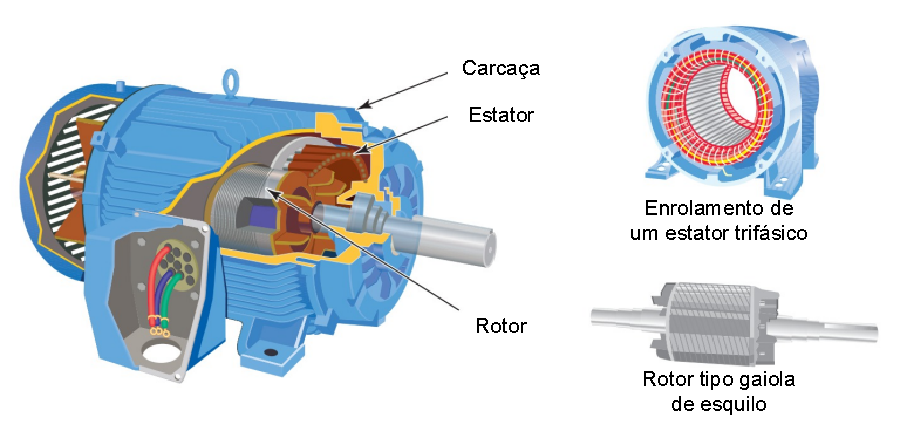
\includegraphics[scale=0.8, page=1]{referencial/img/imagens_referencial.pdf}
    \end{center}
    \fonte{Adaptado de \citeonline{Petruzella1911}.} 
    \label{fig:ind_motor_petruzella_p115}
\end{figure}

Uma das formas de se modelar um motor elétrico de indução, é através de uma representação em forma de um circuito 
elétrico, onde todas as variáveis podem ser representadas por componentes elétricos simples, facilitando a compreensão, modelagem e
prever possíveis variações nos elementos mecânicos e elétricos. O circuito representado na figura \ref{fig:circuit_fitzgerald_p354},
é um circuito equivalente monofásico de um motor elétrico indutivo polifásico, o que simplifica toda a análise em um único circuito,
onde é trivial isolar a tensão em um terminal e a sua corrente. Para se saber as demais correntes e tensões, basta deslocar as fases
em $\pm\ang{120}$ \cite{Umans2003}.

\begin{figure}[H]
    \caption{Circuito equivalente monofásico de um motor de indução polifásico.}
    \begin{center}
        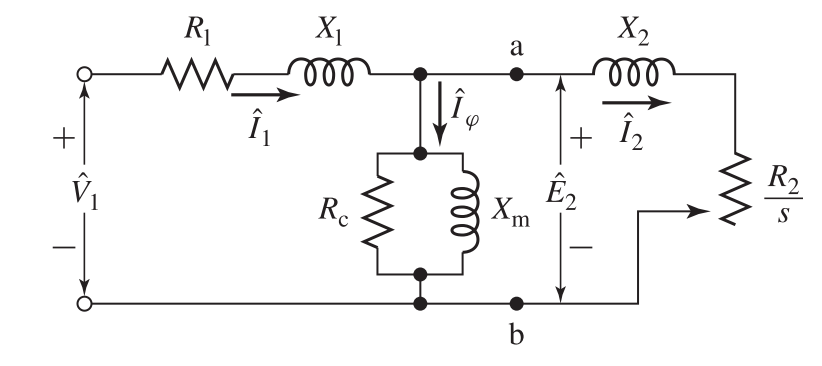
\includegraphics[scale=.35]{referencial/img/circuit_fitzgerald_p354.png}
    \end{center}
    \fonte{\citeonline{Umans2003}.} 
    \label{fig:circuit_fitzgerald_p354}
\end{figure}

Onde

\begin{itemize}
    \item $\hat{V}_1$ = tensão no estator
    \item $\hat{E}_2$ = Força eletromotriz contrária gerada pelo fluxo no entreferro
    \item $\hat{I}_1$ = corrente do estator
    \item $\hat{R}_1$ = resistência efetiva do estator
    \item $\hat{X}_1$ = reatância de vazamento do estator
    \item $R_c$ = resistência às perdas no núcleo
    \item $X_m$ = reatância magnetizante
    \item $\hat{I}_2$ = componente de corrente gerada pela carga
    \item $\hat{X}_2$ = reatância de vazamento do rotor no estator na frequência de escorregamento
    \item $R_2$ = resistência do rotor
    \item $\hat{I}_\varphi$ = componente de corrente excitada no estator
\end{itemize}

Com a apresentação de conceitos básicos sobre motores elétricos de indução e sua modelagem, é possível abordar os principais falhas que 
acometem as partes mecânicas e elétricas de um motor elétrico.


%----------------------------------------------------------------
% 
%----------------------------------------------------------------

\section{Falhas em Motores Elétricos de Indução}\label{sec:}

Como dito anteriormente, um motor elétrico é utilizado para transformar energia elétrica em mecânica, sendo empregado em máquinas que podem
realizar diversas atividades. A figura \ref{fig:monitoring_methods_rilski_p78} representa uma generalização de um sistema em que um motor
elétrico é empregado. Nesta figura, podemos ver os elementos que constituem a parte elétrica: a fonte de energia, o inversor de frequência e
o próprio motor. Também é possível ver a parte mecânica: a estrutura do motor, o acoplamento mecânico, a carga e as bases. Todos esses
elementos podem induzir falhas no motor, começando pelo acionamento, onde pode ocorrer uma falha e fazer o motor perder uma fase, ou ainda, 
oscilações na tensão e sobre carga. Todas essas falhas inevitavelmente alteram o espectro da fonte de energia \citeonline{Gorbounov2018}. 
Na parte mecânica, o desalinhamento entre a carga e o motor pode acarretar falhas no acoplamento que transfere a energia mecânica do motor
para o processo, e isso é normalmente provocado por uma instalação inapropriada.

\begin{figure}[H]
    \caption{Visão geral de sistema com um motor elétrico.}
    \begin{center}
        \includegraphics[scale=0.9, page=2]{referencial/img/imagens_referencial.pdf}
    \end{center}
    \fonte{Adaptado de \citeonline{Gorbounov2018}.} 
    \label{fig:motor_system_rilski_p2}
\end{figure}

A figura \ref{fig:faults_rilski_p77} apresenta uma árvore das principais falhas que acometem os motores elétricos, sendo também divididas
em mecânicas e elétricas. 

\begin{figure}[H]
    \caption{Árvore dos principais tipos de falhas em motores elétricos.}
    \begin{center}
        \includegraphics[scale=1, page=3]{referencial/img/imagens_referencial.pdf}
    \end{center}
    \fonte{Adaptado de \citeonline{Gorbounov2018}.} 
    \label{fig:faults_rilski_p77}
\end{figure}

Dentre todas essas falhas, o trabalho aborda com maior foco as falhas mecânicas, mais especificamente desalinhamento, rolamentos 
e desbalanceamento que causam um aumento na vibração do sistema. O desalinhamento ocorre quando o motor e o sistema não estão perfeitamente alinhados, podendo ter dois tipos:
paralelo e angular, os quais podem ser vistos na figura \ref{fig:misadraw_analog_p2}, respectivamente na parte a) e b) 
\cite{Sopcik2019}.

\begin{figure}[H]
    \caption{Ilustração com os tipos de desalinhamento.}
    \begin{center}
        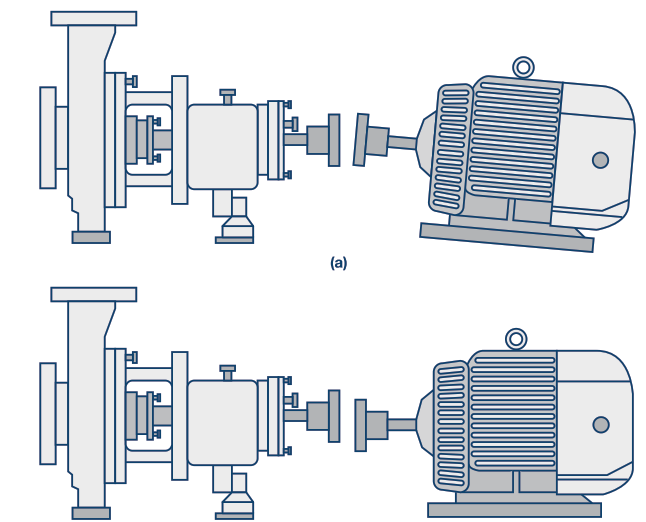
\includegraphics[scale=.35]{referencial/img/misadraw_analog_p2.png}
    \end{center}
    \fonte{\citeonline{Sopcik2019}.} 
    \label{fig:misadraw_analog_p2}
\end{figure}

Já a falha de desbalanceamento, pode ocorrer em qualquer parte rotativa do sistema, que vai desde o motor até a carga, compreendida por
algum problema na disposição das massas. Por último, os rolamentos, que são utilizados em diversas partes de um sistema e que podem
apresentar pequenas rachaduras na falta de lubrificação, que podem ser vistas na figura \ref{fig:bearing_analog_p3}, aumentando a 
vibração \cite{Sopcik2019}.

\begin{figure}[H]
    \caption{Imagens de rolamentos no topo, e falhas na parte de baixo.}
    \begin{center}
        \includegraphics[scale=0.85, page=4]{referencial/img/imagens_referencial.pdf}
    \end{center}
    \fonte{Adaptado de \citeonline{Sopcik2019}.} 
    \label{fig:bearing_analog_p3}
\end{figure}

Mais de 66\% destas falhas são detectadas durante a operação e 28\% são encontradas apenas durante a manutenção 
preventiva \cite{Gorbounov2018}, destacando a importância de uma boa estratégia de manutenção. Existem três tipos de estratégias 
para manutenção \cite{Wu2013}:  

\begin{enumerate}
    \item Funcionar até quebrar: é uma das técnicas mais tradicionais, onde o equipamento funciona até quebrar. Só após isso a
manutenção é realizada. Possui diversas desvantagens, principalmente pelo fato que a falha pode se manifestar durante a produção e
deixar a máquina parada por horas, causando grande prejuízo;
    \item Manutenção Preventiva: é baseada em manutenções em intervalos regulares antes da falha se manifestar. Quando a frequência das
falhas é conhecida, pode ser uma boa estratégia, mas possibilita a troca de componentes que ainda teriam uma sobrevida, ou ainda, a falha
ocorrer antes do previsto, devido à alterações não esperada no processo;
    \item Manutenção Preditiva: quando é detectado que uma falha está próxima, antes de acontecer e com tempo ótimo para se fazer a 
manutenção sem afetar a produtividade e danificar mais o equipamento. Essa estratégia é baseada em um monitoramento do equipamento,
permitindo acompanhar o estado de saúde da máquina. Se bem implementa essa estratégia, pode reduzir em até 65\% os custos de manutenção
\cite{Wu2013};
\end{enumerate}

Após apresentados os conceitos básicos sobre motores elétricos e suas falhas, e como essas falhas aumentam o nível de vibração,
o próximo capítulo tem por objetivo apresentar conceitos de detecção e diagnóstico destas falhas.


%++++++++++++++++++++++++++++++++++++++++++++++++++++++++++++++++
% 
%++++++++++++++++++++++++++++++++++++++++++++++++++++++++++++++++

\section{Sistemas de Detecção e Diagnóstico de Falhas}\label{sec:}

Como apresentado anteriormente, falhas em componentes de um motor elétrico, ou no sistema em que ele está inserido, podem ocasionar
um aumento da vibração e alteração no espectro da corrente do motor, que serão estudados na sequência.


%----------------------------------------------------------------
% 
%----------------------------------------------------------------

\subsection{Análise de Vibração}\label{subsec:}

O aumento da vibração pode ocasionar perturbações até mesmo na parte elétrica de um motor, como mostra o gráfico que está na 
figura \ref{fig:fault_effect_randall_p54}. Com o aumento da carga e da vibração em conjunto, o efeito mecânico e elétrico pode ser 
severo \citeonline{Wu2013}.

\begin{figure}[H]
    \caption{Variação da carga para distinção da causa do efeito observado.}
    \begin{center}
        \includegraphics[scale=0.8, page=5]{referencial/img/imagens_referencial.pdf}
    \end{center}
    \fonte{Adaptado de \citeonline{Wu2013}.} 
    \label{fig:fault_effect_randall_p54}
\end{figure}


Essa vibração possui um característica específica, que depende de qual falha ela é oriunda, que acaba criando uma assinatura
ao se analisar a vibração, sendo possível diagnosticar se o motor e o sistema em que ele está inserido está com boa saúde \cite{Wu2013}.
Uma das primeiras técnicas para classificar o estado de saúde de uma máquina, é a norma ISO 10816-1, que recomenda níveis de vibração 
em valores eficaz de acordo com o porte da máquina, que pode ser visto na figura \ref{fig:iso10816-1_randall_p146}.

\begin{table}[H]
    \caption{Tabela de valores eficaz máximos de velocidade para cada porte de máquina indicados pela norma ISO 10816-1.}
    \label{tab:iso10816-1_randall_p146}
    \centering%
    \begin{minipage}{.9\textwidth}
        \begin{tabular*}{\textwidth}{|c|c|c|c|c|}
            \hline
            \multicolumn{1}{|c|}{Velocidade de vibração RMS [\SI{}{\milli\metre\per\second}] }& Classe I                                                         & Classe II                                                        & Classe III                                                       & Classe IV                                                        \\ \hline
            \multicolumn{1}{|c|}{0.25}            & \multicolumn{1}{c|}{\cellcolor[HTML]{00FF02}}                    & \multicolumn{1}{c|}{\cellcolor[HTML]{00FF02}}                    & \multicolumn{1}{c|}{\cellcolor[HTML]{00FF02}}                    & \multicolumn{1}{c|}{\cellcolor[HTML]{00FF02}}                    \\ \cline{1-1}
            \multicolumn{1}{|c|}{0.45}            & \multicolumn{1}{c|}{\cellcolor[HTML]{00FF02}}                    & \multicolumn{1}{c|}{\cellcolor[HTML]{00FF02}}                    & \multicolumn{1}{c|}{\cellcolor[HTML]{00FF02}}                    & \multicolumn{1}{c|}{\cellcolor[HTML]{00FF02}}                    \\ \cline{1-1}
            \multicolumn{1}{|c|}{0.71}            & \multicolumn{1}{c|}{\multirow{-3}{*}{\cellcolor[HTML]{00FF02}A}} & \multicolumn{1}{c|}{\cellcolor[HTML]{00FF02}}                    & \multicolumn{1}{c|}{\cellcolor[HTML]{00FF02}}                    & \multicolumn{1}{c|}{\cellcolor[HTML]{00FF02}}                    \\ \cline{1-2}
            \multicolumn{1}{|c|}{1.12}            & \multicolumn{1}{c|}{\cellcolor[HTML]{00D2CB}}                    & \multicolumn{1}{c|}{\multirow{-4}{*}{\cellcolor[HTML]{00FF02}A}} & \multicolumn{1}{c|}{\cellcolor[HTML]{00FF02}}                    & \multicolumn{1}{c|}{\cellcolor[HTML]{00FF02}}                    \\ \cline{1-1} \cline{3-3}
            \multicolumn{1}{|c|}{1.8}             & \multicolumn{1}{c|}{\multirow{-2}{*}{\cellcolor[HTML]{00D2CB}B}} & \multicolumn{1}{c|}{\cellcolor[HTML]{00D2CB}}                    & \multicolumn{1}{c|}{\multirow{-5}{*}{\cellcolor[HTML]{00FF02}A}} & \multicolumn{1}{c|}{\cellcolor[HTML]{00FF02}}                    \\ \cline{1-2} \cline{4-4}
            \multicolumn{1}{|c|}{2.8}             & \multicolumn{1}{c|}{\cellcolor[HTML]{F8FF00}}                    & \multicolumn{1}{c|}{\multirow{-2}{*}{\cellcolor[HTML]{00D2CB}B}} & \multicolumn{1}{c|}{\cellcolor[HTML]{00D2CB}}                    & \multicolumn{1}{c|}{\multirow{-6}{*}{\cellcolor[HTML]{00FF02}A}} \\ \cline{1-1} \cline{3-3} \cline{5-5} 
            \multicolumn{1}{|c|}{4.5}             & \multicolumn{1}{c|}{\multirow{-2}{*}{\cellcolor[HTML]{F8FF00}C}} & \multicolumn{1}{c|}{\cellcolor[HTML]{F8FF00}}                    & \multicolumn{1}{c|}{\multirow{-2}{*}{\cellcolor[HTML]{00D2CB}B}} & \multicolumn{1}{c|}{\cellcolor[HTML]{00D2CB}}                    \\ \cline{1-2} \cline{4-4}
            \multicolumn{1}{|c|}{7.1}             & \multicolumn{1}{c|}{\cellcolor[HTML]{FE0000}}                    & \multicolumn{1}{c|}{\multirow{-2}{*}{\cellcolor[HTML]{F8FF00}C}} & \multicolumn{1}{c|}{\cellcolor[HTML]{F8FF00}}                    & \multicolumn{1}{c|}{\multirow{-2}{*}{\cellcolor[HTML]{00D2CB}B}} \\ \cline{1-1} \cline{3-3} \cline{5-5} 
            \multicolumn{1}{|c|}{11.2}            & \multicolumn{1}{c|}{\cellcolor[HTML]{FE0000}}                    & \multicolumn{1}{c|}{\cellcolor[HTML]{FE0000}}                    & \multicolumn{1}{c|}{\multirow{-2}{*}{\cellcolor[HTML]{F8FF00}C}} & \multicolumn{1}{c|}{\cellcolor[HTML]{F8FF00}}                    \\ \cline{1-1} \cline{4-4}
            \multicolumn{1}{|c|}{18}              & \multicolumn{1}{c|}{\cellcolor[HTML]{FE0000}}                    & \multicolumn{1}{c|}{\cellcolor[HTML]{FE0000}}                    & \multicolumn{1}{c|}{\cellcolor[HTML]{FE0000}}                    & \multicolumn{1}{c|}{\multirow{-2}{*}{\cellcolor[HTML]{F8FF00}C}} \\ \cline{1-1} \cline{5-5} 
            \multicolumn{1}{|c|}{28}              & \multicolumn{1}{c|}{\cellcolor[HTML]{FE0000}}                    & \multicolumn{1}{c|}{\cellcolor[HTML]{FE0000}}                    & \multicolumn{1}{c|}{\cellcolor[HTML]{FE0000}}                    & \multicolumn{1}{c|}{\cellcolor[HTML]{FE0000}}                    \\ \cline{1-1} \cline{5-5} 
            \multicolumn{1}{|c|}{45}              & \multicolumn{1}{c|}{\multirow{-5}{*}{\cellcolor[HTML]{FE0000}D}} & \multicolumn{1}{c|}{\multirow{-4}{*}{\cellcolor[HTML]{FE0000}D}} & \multicolumn{1}{c|}{\multirow{-3}{*}{\cellcolor[HTML]{FE0000}D}} & \multicolumn{1}{c|}{\multirow{-2}{*}{\cellcolor[HTML]{FE0000}D}} \\ \cline{1-1} \cline{5-5}
        \end{tabular*}
      \fonte{Adaptado de \citeonline{Wu2013}.} 
    \end{minipage}
  \end{table}

Onde

\begin{itemize}
    \item A = bom estado
    \item B = aceitável
    \item C = apenas tolerável
    \item D = não permitido
    \item Classe I = pequenas máquinas (potência menor que $\SI{15}{\kilo\watt}$)
    \item Classe II = máquinas médias sem uma fundação especial (potência entre $\SI{15}{\kilo\watt}$ e $\SI{75}{\kilo\watt}$)
    \item Classe III = máquinas grandes sobre uma fundação rígida e pesada
    \item Classe IV = máquinas grandes sobre uma fundação flexível (turbomáquinas) 
\end{itemize}

Relembrando o que foi escrito anteriormente, é possível ver as assinaturas das falhas no espectro da vibração captada por um transdutor
que está acoplado no sistema. Quando uma falha de desalinhamento está presente, há um aumento de até duas vezes nas harmônicas de alta 
frequência, como pode ser visto na figura \ref{fig:misa_analog_p2} \cite{Sopcik2019}.

\begin{figure}[H]
    \caption{Indicação espectral de desalinhamento na velocidade.}
    \begin{center}
        \includegraphics[scale=0.7, page=6]{referencial/img/imagens_referencial.pdf}
    \end{center}
    \fonte{Adaptado de \citeonline{Sopcik2019}.} 
    \label{fig:misa_analog_p2}
\end{figure}

Já quando uma falha de desbalanceamento está presente, há um aumento na harmônica principal da velocidade, em relação ao valor de base.
A figura \ref{fig:imbalance_analog_p2} exemplifica.

\begin{figure}[H]
    \caption{Indicação espectral de desbalanceamento na velocidade.}
    \begin{center}
        \includegraphics[scale=0.8, page=7]{referencial/img/imagens_referencial.pdf}
    \end{center}
    \fonte{Adaptado de \citeonline{Sopcik2019}.} 
    \label{fig:imbalance_analog_p2}
\end{figure}

No mesmo conceito, é possível identificar a assinatura de uma falha de rolamentos de acordo com o tipo de rolamento, velocidade de rotação
do motor, entre outras características. Após a análise das falhas utilizando a vibração do sistema, é necessário fazer a mesma análise com a corrente elétrica na armadura, 
que será apresenta na subseção na sequência.



%++++++++++++++++++++++++++++++++++++++++++++++++++++++++++++++++
% 
%++++++++++++++++++++++++++++++++++++++++++++++++++++++++++++++++

\section{Técnicas Modernas de Processamento de Sinais}\label{sec:}

Com o objetivo de se detectar falhas e se obter um diagnóstico das mesmas, muitas técnicas já foram implementadas. Essas técnicas podem ser
não invasivas ou invasivas \cite{Gorbounov2018}. A figura \ref{fig:monitoring_methods_rilski_p78} apresenta algumas técnicas que são
utilizadas para detecção e diagnóstico de falhas.

\begin{figure}[H]
    \caption{Árvore de métodos de monitoramento de falhas em motores elétricos.}
    \begin{center}
        \includegraphics[scale=0.9, page=8]{referencial/img/imagens_referencial.pdf}
    \end{center}
    \fonte{Adaptado de \citeonline{Gorbounov2018}.} 
    \label{fig:monitoring_methods_rilski_p78}
\end{figure}

Dentre essas, a FFT (\textit{Fast Fourier Transform - transformada rápida de Fourier}), que será descritas na sequência, 
adicionando mais uma técnica de análise de assinaturas que é a ICA (\textit{Indepent Compoent Analysys} - análise de componentes independentes).
Além disso, o presente trabalho também aborda duas técnicas de aprendizado de máquina, que  é a t-SNE 
(\textit{t-Distributed Stochastic Neighbor Embedding} - Incorporação Estocástica de Vizinhos com Distribuição t) e, por último, 
 a técnica K-means.


%----------------------------------------------------------------
% 
%----------------------------------------------------------------

\subsection{Aprendizado de Máquina}


<<< estatística e algumas regras>>>


%++++++++++++++++++++++++++++++++++++++++++++++++++++++++++++++++
% 
%++++++++++++++++++++++++++++++++++++++++++++++++++++++++++++++++

\section{Estado da Arte}

O estado da arte em detecção e diagnóstico de falhas em motores elétricos está no emprego de diversas técnicas numa mesma solução. Algumas 
utilizam técnicas clássicas, outras empregam diversas técnicas modernas para se obter o resultado ótimo. A presente seção contem
algum exemplos que empregam novos arranjos de técnicas, as quais já foram discutidas anteriormente.


%----------------------------------------------------------------
% 
%----------------------------------------------------------------

\subsection{Aprendizado de Máquina}


<<< estatística e algumas regras aplicada a vibração (meu código implementado)>>>